\hsection{Installing Psycopg}%
\label{sec:installPsycopg}%
%
\begin{figure}%
\centering%
%
\subfloat[][%
We first open a \pgls{terminal} using \ubuntuTerminal.
We navigate to the directory where our programming will take place. %
We now create a directory \textil{.venv} to host a new \pgls{virtualEnvironment} by typing \bashil{mkdir .venv} and hitting~\keys{\enter}.%
\label{fig:pipInstallPyscopgVenv1mkdir}%
]{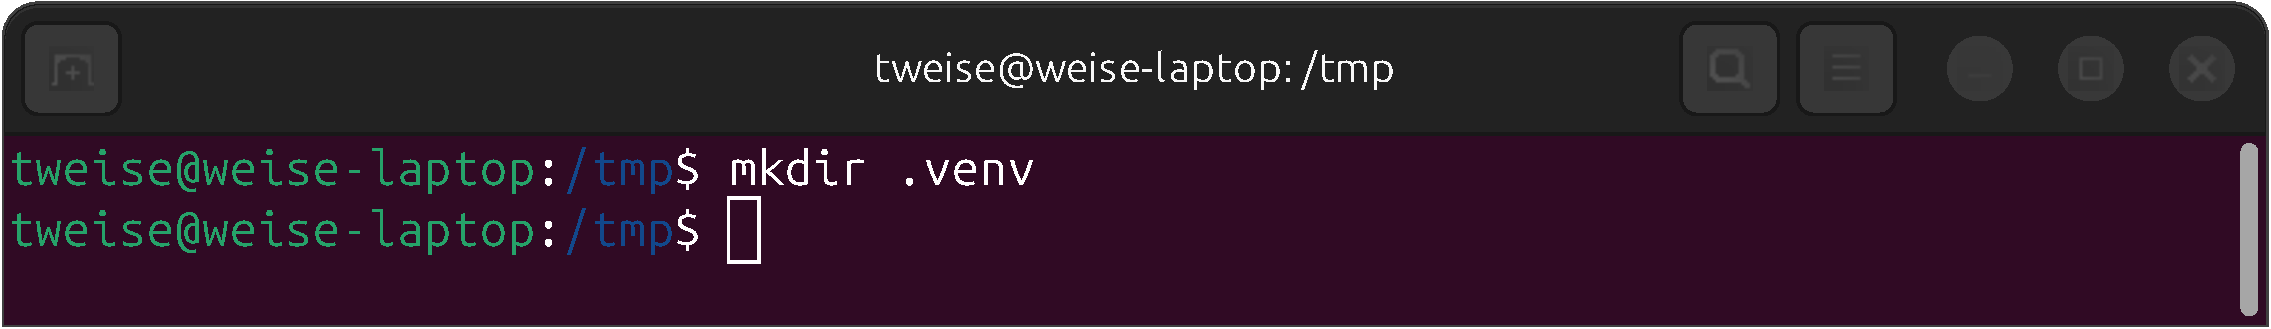
\includegraphics[width=0.7\linewidth]{\currentDir/pipInstallPyscopgVenv1mkdir}}%
%
\floatRowSep%
%
\subfloat[][%
We now set up a new and empty \pgls{virtualEnvironment} in this directory by writing \bashil{python3 -m venv --upgrade-deps .venv} and hitting~\keys{\enter}.%
\label{fig:pipInstallPyscopgVenv2venv}%
]{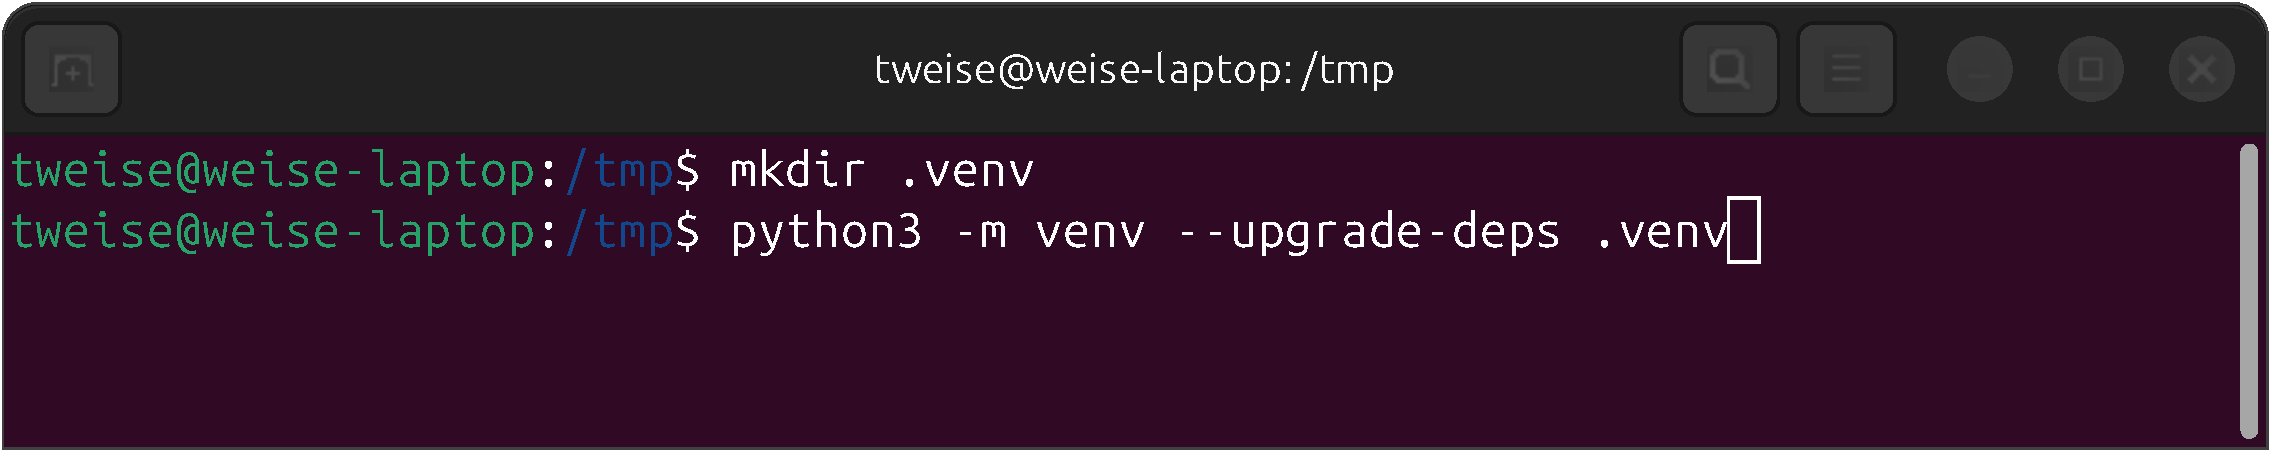
\includegraphics[width=0.7\linewidth]{\currentDir/pipInstallPyscopgVenv2venv}}%
%
\floatRowSep%
%
\subfloat[][%
The \pgls{virtualEnvironment} has been created. %
We now activate it by writing \bashil{source .venv/bin/activate} and hitting~\keys{\enter}.%
\label{fig:pipInstallPyscopgVenv3activate}%
]{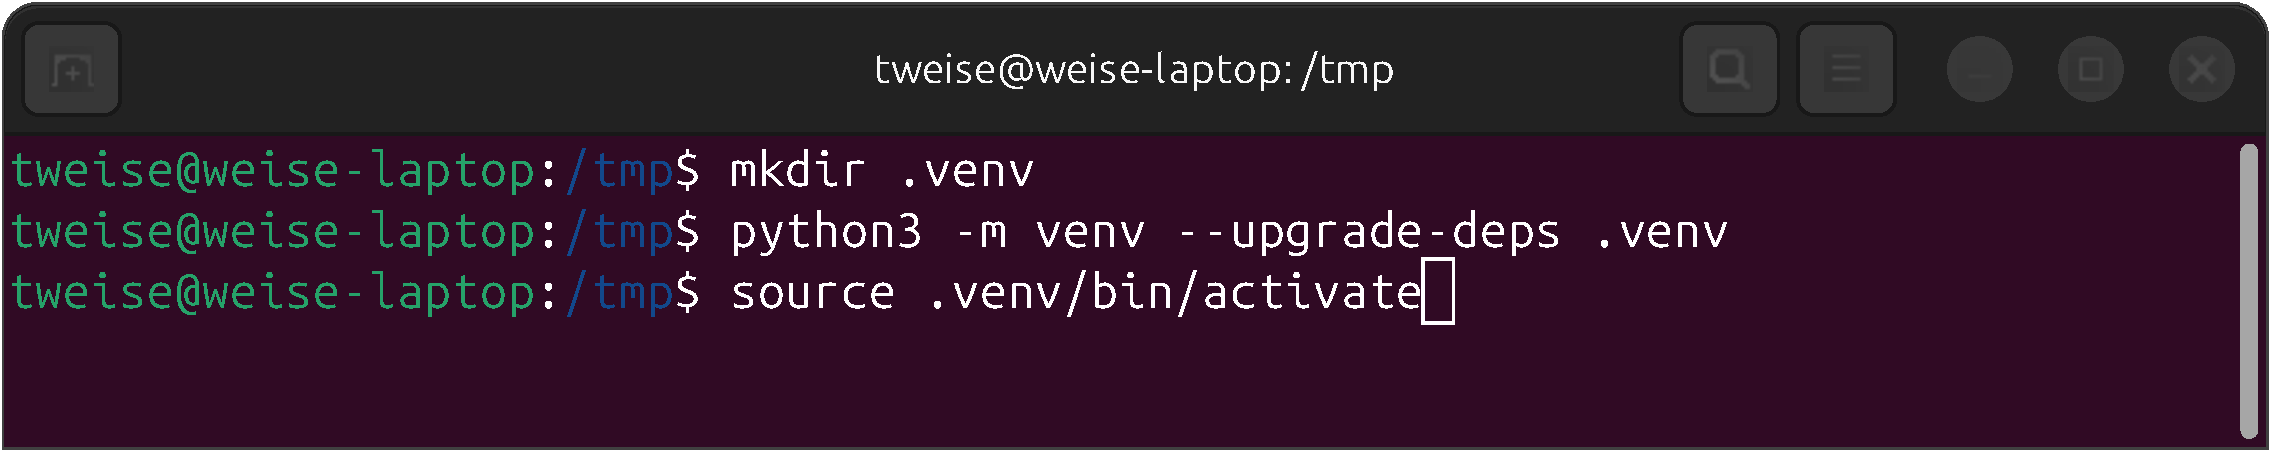
\includegraphics[width=0.7\linewidth]{\currentDir/pipInstallPyscopgVenv3activate}}%
%
\floatRowSep%
%
\subfloat[][%
The \pgls{virtualEnvironment} \textil{.venv} is now active, which we can see by the changed prompt.%
\label{fig:pipInstallPyscopgVenv4activated}%
]{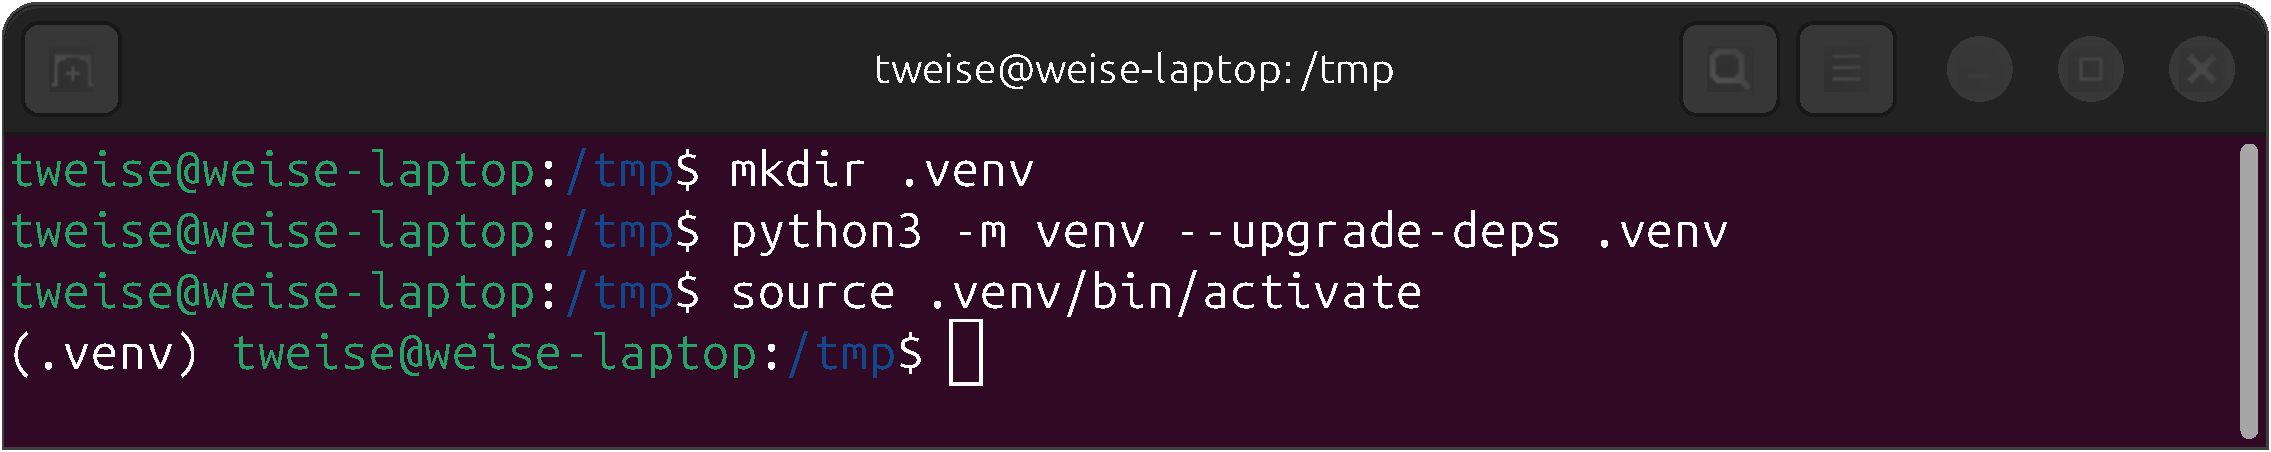
\includegraphics[width=0.7\linewidth]{\currentDir/pipInstallPyscopgVenv4activated}}%
%
\floatRowSep%
%
\subfloat[][%
We install \psycopg\ into this environment by writing \bashil{pip install psycopg} and hitting~\keys{\enter}.%
\label{fig:pipInstallPyscopgVenv5pip}%
]{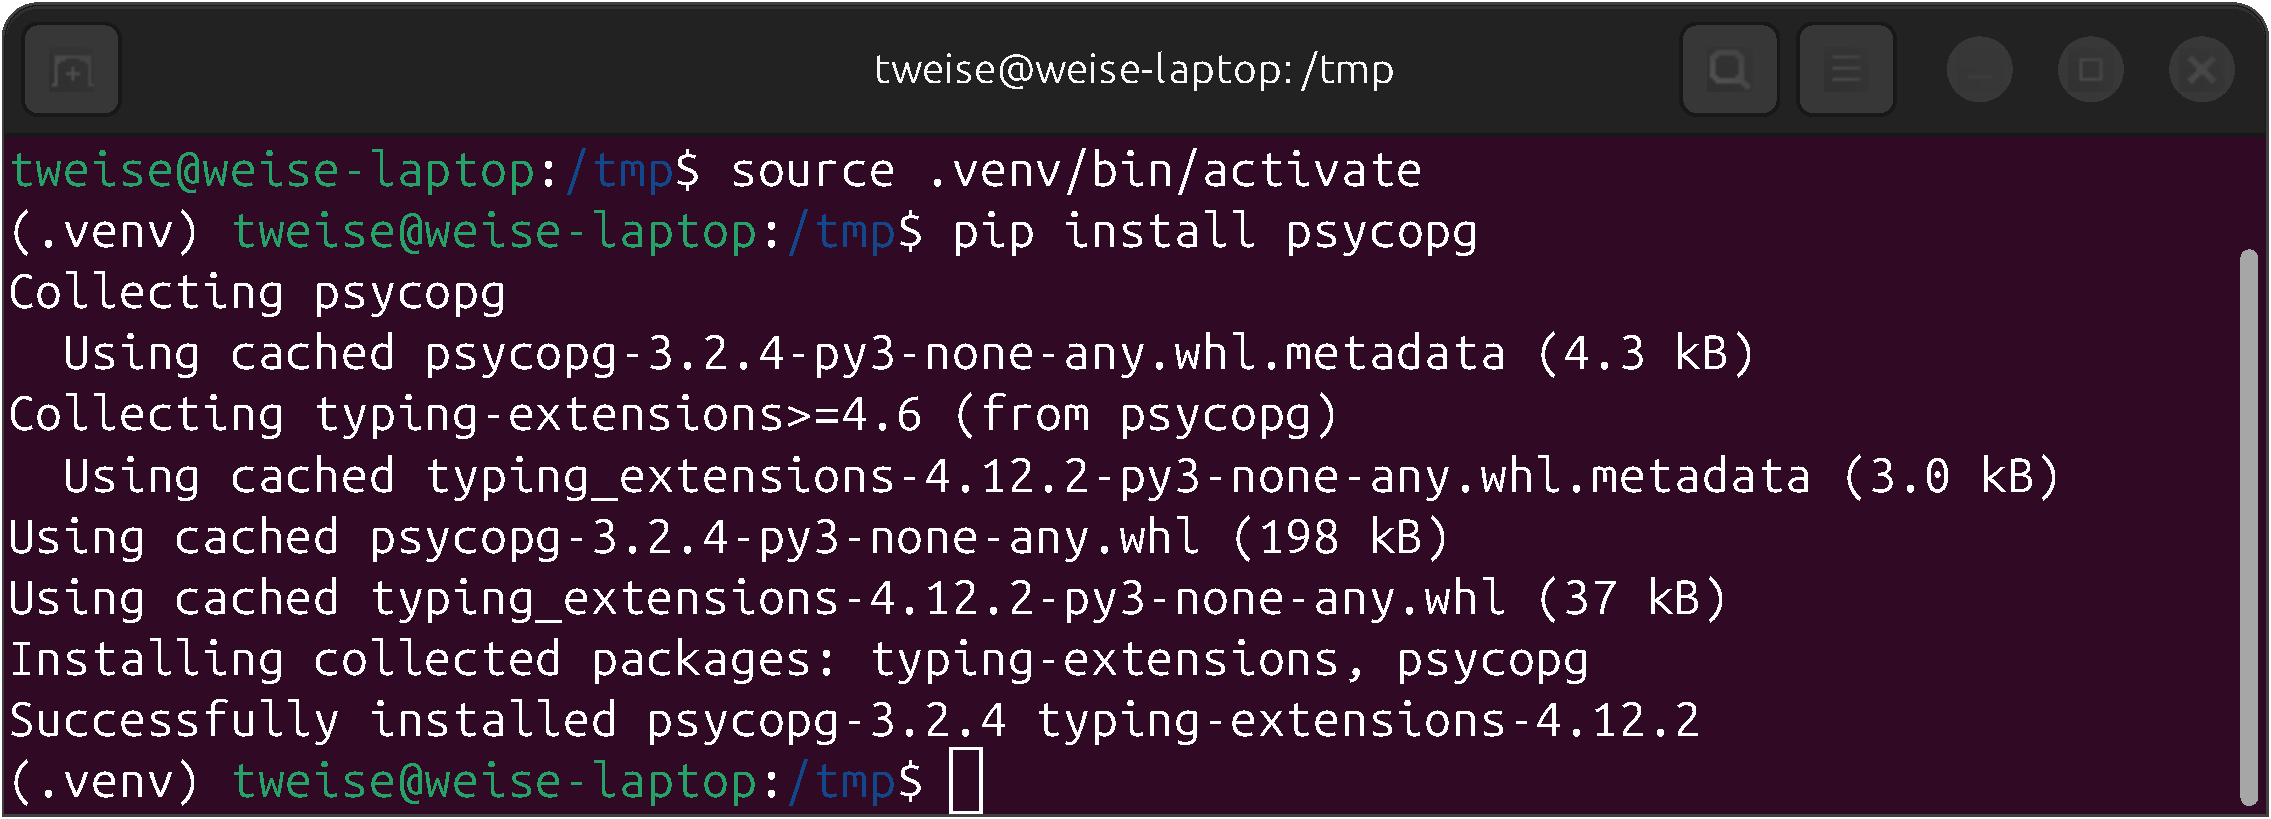
\includegraphics[width=0.7\linewidth]{\currentDir/pipInstallPyscopgVenv5pip}}%
%
\floatRowSep%
%
\subfloat[][%
Once we have finished programming, we can deactivate the \pgls{virtualEnvironment} by writing~\bashil{deactivate} and hitting~\keys{\enter}. %
The prompt changes back to normal.%
\label{fig:pipInstallPyscopgVenv6deactivate}%
]{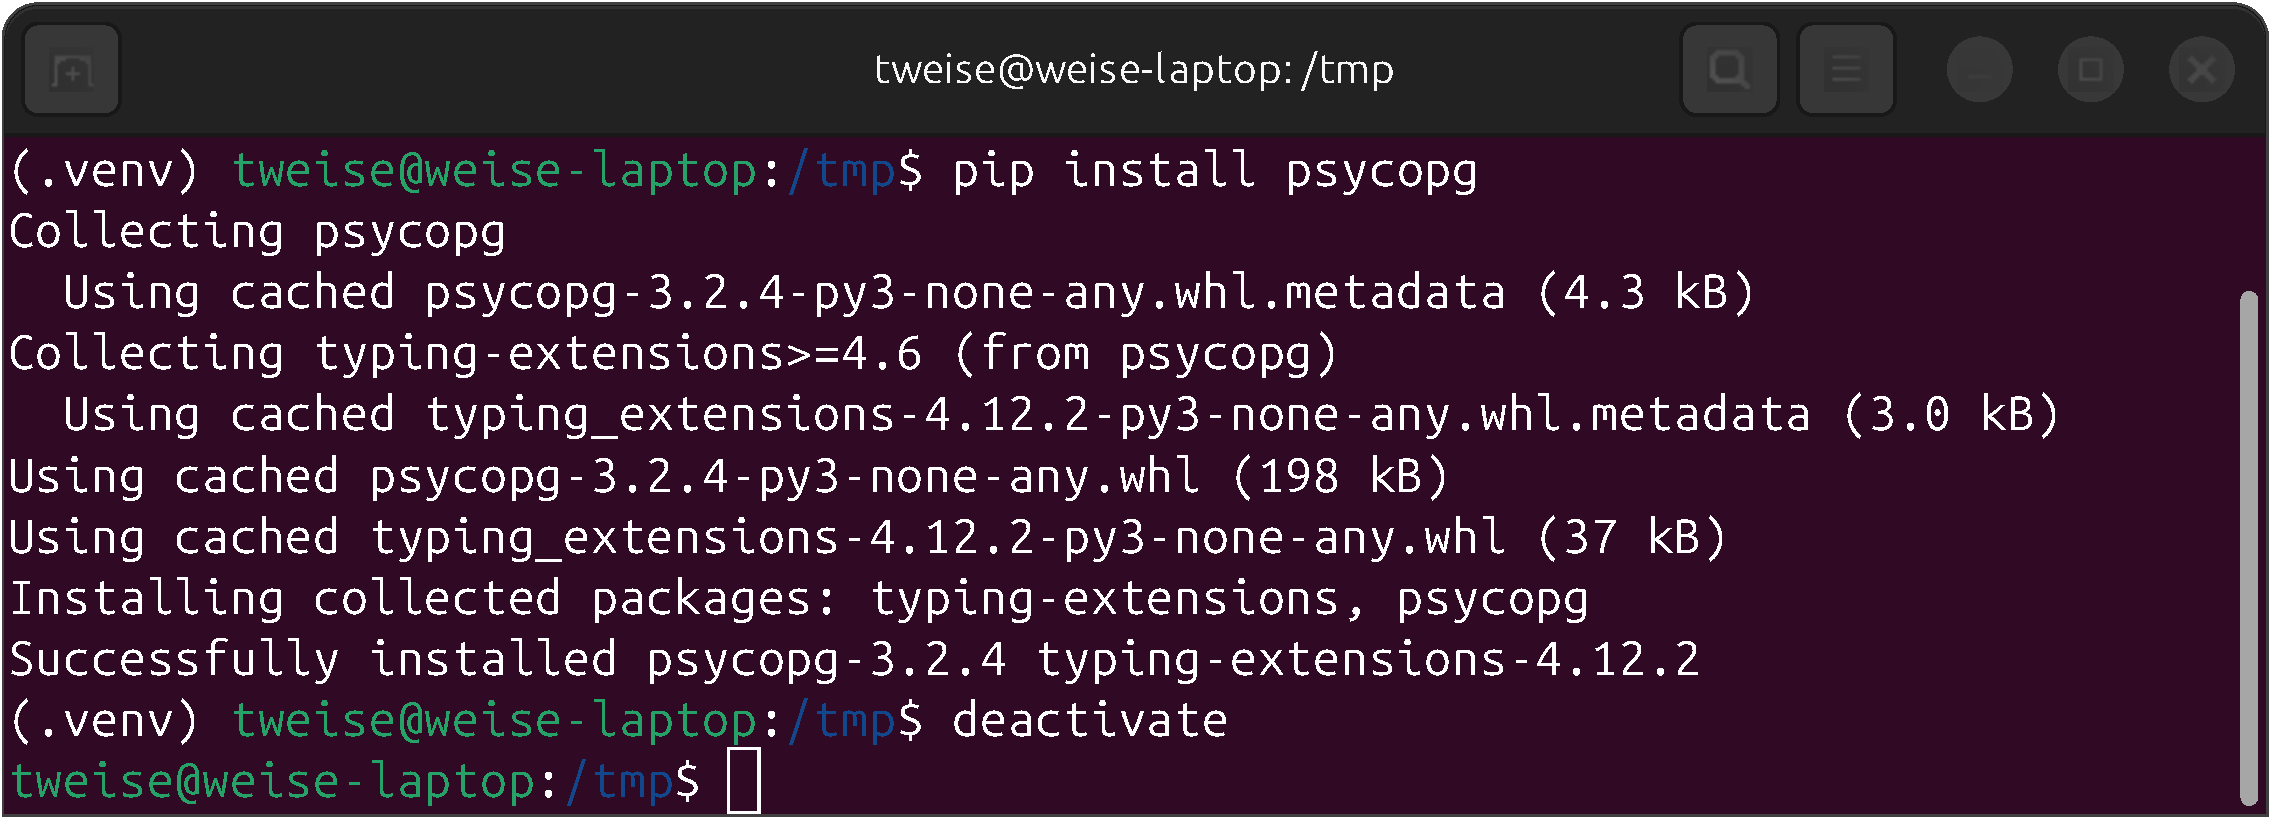
\includegraphics[width=0.7\linewidth]{\currentDir/pipInstallPyscopgVenv6deactivate}}%
%
\caption{Installing the \python\ package \psycopg\ into a \pgls{virtualEnvironment} under \ubuntu\ \linux\ using \pip\ in a \bash\ shell \pgls{terminal}.}%
\label{fig:installPsycopgLinux}%
%
\end{figure}%
%
Since the installation of the programming language \python\ and the \pgls{ide} \pycharm\ is already covered in~\cite{programmingWithPython}, we will not reproduce this information here.
The download of our examples and the setup of the required \psycopg\ library in a \pgls{virtualEnvironment} in \pycharm\ is \emph{also} covered in~\cite{programmingWithPython}.
For the sake of completeness, we will therefore only briefly iterate over the installation of \psycopg\ using \pip\ at this stage.
It is assumed, however, that you have read~\cite{programmingWithPython} at least to a point where you know what \pip\ is and what \pglspl{virtualEnvironment} are.
We also cover the installation only under \ubuntu\ \linux, as the installation steps under \microsoftWindows\ will be analogous (see again~\cite{programmingWithPython}).

The most common way to use external packages in \python\ is to install them into \pglspl{virtualEnvironment}.
A \pgls{virtualEnvironment} is essentially something like a directory hosting a stand-alone \python\ installation separate from the \python\ setup of the computer.
This allows you to have different versions of different libraries installed (in different \pglspl{virtualEnvironment}).

Imagine that you have one program that requires the \python\ package \numpy\ in version~2.0 or above to run.
You also need to use another application, which can only run with \numpy\ \emph{below} version~2.0.
This is a very common scenario.
It would be impossible to realize, because you can only have one version of \numpy\ installed in your system.
However, you can use both applications if each is installed into its own \pgls{virtualEnvironment}.
Because each \pgls{virtualEnvironment} can have its own version of \numpy.

Therefore, we will explore this route of installing packages, and we will do so under \ubuntu\ \linux\ in the \bash\ \pgls{terminal} in \cref{fig:installPsycopgLinux}.
For \microsoftWindows, you can find a similar procedure discussed in~\cite{programmingWithPython}.
The commands there are almost the same.

We begin by open a \bash\ \pgls{terminal} using \ubuntuTerminal.
Then we navigate to the directory where our programming will take place.
In my example, I chose the temporary directory \bashil{/tmp} because I will delete everything once I am done taking screenshots.
You would choose a more sensible location.
Inside this directory, we now create a new directory \textil{.venv} to host a new \pgls{virtualEnvironment}.
In the \bash\ shell, we can do this by typing the command \bashil{mkdir .venv} and hitting~\keys{\enter} in \cref{fig:pipInstallPyscopgVenv1mkdir}

After this empty new directory is created, we can instruct \python\ to prepare it for use as a \pgls{virtualEnvironment} in \cref{fig:pipInstallPyscopgVenv2venv}.
We set up a new and empty \pgls{virtualEnvironment} in this directory by writing \bashil{python3 -m venv --upgrade-deps .venv} and hitting~\keys{\enter}.
The new \pgls{virtualEnvironment} has been created.
We now activate it by writing \bashil{source .venv/bin/activate} and hitting~\keys{\enter} in \cref{fig:pipInstallPyscopgVenv3activate}.
Once a \pgls{virtualEnvironment} is active, all package installations will go into that environment.
Also, if we run a \python\ program, it will search for installed packages in this environment.
And our \pgls{virtualEnvironment} \textil{.venv} is now active, which we can see by the changed prompt in \cref{fig:pipInstallPyscopgVenv4activated}.
Notice that the environment is only active in the current \pgls{terminal}.
If you open another \pgls{terminal} using \ubuntuTerminal, our \pgls{virtualEnvironment} is not active in it (but we can activate it exactly as shown in \cref{fig:pipInstallPyscopgVenv3activate}).

We install \psycopg\ into this environment by writing \bashil{pip install psycopg} and hitting~\keys{\enter}.
This invokes the \pip\ installer, which looks the package up in \pypi\ and downloads it.
In \cref{fig:pipInstallPyscopgVenv5pip}, you see that it downloads \psycopg\ in version~\textil{3.2.4}.
When you do the same thing, you will probably get a newer version installed.

If we run a \python\ program that uses \psycopg, like \cref{lst:factory:connect_insert_and_select}, it will find this version of the package in our \pgls{virtualEnvironment}.
Once we have finished programming and running programs, we can deactivate the \pgls{virtualEnvironment} by writing~\bashil{deactivate} and hitting~\keys{\enter}.
The prompt changes back to normal in \cref{fig:pipInstallPyscopgVenv6deactivate}.
Whenever we need \psycopg\ again, we would activate the \pgls{virtualEnvironment} again as shown in \cref{fig:pipInstallPyscopgVenv3activate}.
Of course, we can also install more packages into this environment.
And we can also create more environments if we want to, in the same way as discussed here.%
%
\endhsection%
%
